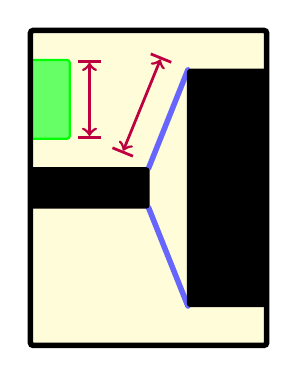
\begin{tikzpicture}[thick,scale=.5, every node/.style={scale=1}]

\begin{scope}

\clip (0,0) -- (6,0) -- (6,8) -- (0,8) -- cycle;

\draw [line width=0,fill=yellow!15!white] (0,0) -- (6,0) -- (6,8) -- (0,8) -- cycle;

\draw [blue!60!white,line width=2,line cap=round] (4,7) -- (3,4.5);
\draw [blue!60!white,line width=2,line cap=round] (4,1) -- (3,3.5);

\draw [fill=black,rounded corners=1] (4,7) -- (6,7) -- (6,1) -- (4,1) -- cycle;
\draw [fill=black,rounded corners=1] (0,4.5) -- (3,4.5) -- (3,3.5) -- (0,3.5) -- cycle;

\draw [green,fill=green!60!white,rounded corners=1,shift={(1,2.25)}] (-3,3) -- (-3,5) -- (0,5) -- (0,3) -- cycle;

\draw [arrows=|<->|,purple,line width=1pt,line cap=round,shift={(1,2.25)}] (0.5,5) -- (0.5,3);
\draw [arrows=|<->|,purple,line width=1pt,line cap=round] (3.33,7.33) -- (2.33,4.88);

\end{scope}

\draw [line width=2,rounded corners=1] (0,0) -- (6,0) -- (6,8) -- (0,8) -- cycle;

\end{tikzpicture}